%
% tetraeder.tex
%
% (c) 2017 Prof Dr Andreas Müller, Hochschule Rapperswil
%
\subsection{Tetraeder}
% XXX 3D-Darstellung  
Ein Tetraeder besteht aus vier Dreiecken, die an den Kanten verbunden
sind.
Es hat vier Ecken, vier Seitenflächen und sechs Kanten.
Der Eulersche Polyeder-Satz sagt, dass 
\[
e-f+k = 4+6-4=2,
\]
für jedes andere geschlosene Polyeder auch.

\begin{figure}
\centering
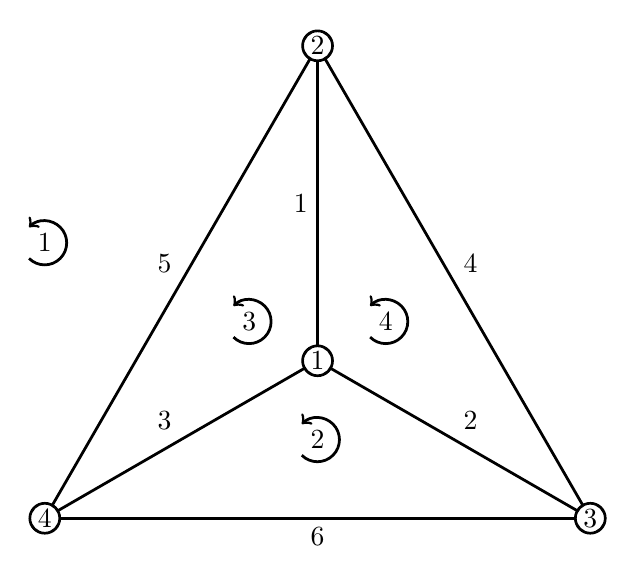
\begin{tikzpicture}[scale=4]

\coordinate (A) at (0,0);
\coordinate (B) at (0,1);
\coordinate (C) at (0.866,-0.5);
\coordinate (D) at (-0.866,-0.5);

\coordinate (b) at (0,-0.25);
\coordinate (c) at (-0.217,0.125);
\coordinate (d) at (0.217,0.125);
\coordinate (a) at (-0.866,0.375);

\coordinate (E) at (0,0.5);
\coordinate (F) at (0.433,-0.25);
\coordinate (G) at (-0.433,-0.25);
\coordinate (H) at (0.433,0.25);
\coordinate (I) at (-0.433,0.25);
\coordinate (J) at (0,-0.5);

\draw[line width=1pt] (A)--(B);
\draw[line width=1pt] (A)--(C);
\draw[line width=1pt] (A)--(D);
\draw[line width=1pt] (B)--(C);
\draw[line width=1pt] (B)--(D);
\draw[line width=1pt] (C)--(D);

\draw[fill=black] (A) circle[radius=0.5mm,fill]{};
\draw[fill=white] (A) circle[radius=0.45mm,fill]{};
\node at (A) {$1$};

\draw[fill=black] (B) circle[radius=0.5mm,fill]{};
\draw[fill=white] (B) circle[radius=0.45mm,fill]{};
\node at (B) {$2$};

\draw[fill=black] (C) circle[radius=0.5mm,fill]{};
\draw[fill=white] (C) circle[radius=0.45mm,fill]{};
\node at (C) {$3$};

\draw[fill=black] (D) circle[radius=0.5mm,fill]{};
\draw[fill=white] (D) circle[radius=0.45mm,fill]{};
\node at (D) {$4$};

\node at (b) {$2$};
\draw[->,line width=1pt] (b) + (-0.5mm,-0.5mm)
	arc[x radius=0.7mm,y radius=0.7mm,start angle=-135,end angle=135];
\node at (c) {$3$};
\draw[->,line width=1pt] (c) + (-0.5mm,-0.5mm)
	arc[x radius=0.7mm,y radius=0.7mm,start angle=-135,end angle=135];
\node at (d) {$4$};
\draw[->,line width=1pt] (d) + (-0.5mm,-0.5mm)
	arc[x radius=0.7mm,y radius=0.7mm,start angle=-135,end angle=135];
\node at (a) {$1$};
\draw[->,line width=1pt] (a) + (-0.5mm,-0.5mm)
	arc[x radius=0.7mm,y radius=0.7mm,start angle=-135,end angle=135];

\node at (E) [left] {$1$};
\node at (F) [above right] {$2$};
\node at (G) [above left] {$3$};
\node at (H) [above right] {$4$};
\node at (I) [above left] {$5$};
\node at (J) [below] {$6$};

\end{tikzpicture}
\caption{Netzwerk eines Tetraeders
\label{homologie:fig:tetragrid}}
\end{figure}

Wir berechnen die Homologie-Vektorräume für ein Tetraeder.
Ein Tetraeder besteht aus vier Dreiecken, die an den Kanten
verbunden sind.
In Abbildung~\ref{homologie:fig:tetragrid} ist das Tetraeder
schematisch dargestellt.
Die Seitenflächen sind numeriert mit den Zahlen, die von kreisförmligen
Pfeilen umgeben sind, die Seitenfläche $1$ soll man sich als die Bodenfläch
des Tetraeders vorstellen.
Die Kanten sind immer von der Ecke mit der kleineren Nummer zur
Ecke mit der grösseren Nummer orientiert.
Die Orientierung der Seitenflächen ist durch die kreisförmigen Pfeile
gegeben.

Aus dem Netzwerk~\ref{homologie:fig:tetragrid} können wir jetzt die
Randoperatoren ableiten.
Der Randoperator $\partial_1$ kann als $4\times 6$-Matrix dargestellt sind,
mit einer Zeile für jede Ecke und einer Spalte für jede Kante des
Tetraeders.
Anfangspunkte einer Kante werden mit $-1$ markiert, Endpunkte mit $1$.
So entsteht die Matrix
\[
\partial_1
=
\begin{pmatrix}
-1&-1&-1& 0& 0& 0\\
 1& 0& 0&-1&-1& 0\\
 0& 1& 0& 1& 0&-1\\
 0& 0& 1& 0& 1& 1
\end{pmatrix}.
\] 
Da die Summe jeder Spalten $0$ ist, kann $\partial_1$ nicht vollen Rang
haben.
Durch Nachrechnen findet man, dass $\operatorname{Rang}\partial_1=3$.

Der Randoperator $\partial_2$ berechnet aus jeder Seitenfläche die Summe
der orientierten Kanten, die die Seitenfläche beranden.
Wir können $\partial_2$ codieren als $6\times 4$-Matrix mit einer Zeile
für jede Kante und einer Spalte für jede Seitenfläche.
Die Kanten, die eine Seitenfläche beranden, werden mit $1$ markiert,
wenn ihre Orientierung mit der Pfeilrichtung der Seitenfläche übereinstimmt.
So erhalten wir die Matrix
\[
\partial_2
=
\begin{pmatrix}
 0& 0& 1&-1\\
 0&-1& 0& 1\\
 0& 1&-1& 0\\
 1& 0& 0&-1\\
-1& 0& 1& 0\\
 1&-1& 0& 0
\end{pmatrix}.
\]
Auch diese Matrix kann nicht vollen Rang haben, da jede Zeilensumme $0$ ist.
Tatsächlich zeigt die Rechnung dass $\operatorname{Rang}\partial_2 = 3$.

Durch Nachrechnen kann man auch kontrollieren, dass $\partial_1\partial_2=0$,
wie man das für einen Randoperator erwartet.
Daher ist $\operatorname{im}\partial_2\subset \operatorname{ker}\partial_1$.
Wir können jetzt die Dimensionen von Kern und Bild jedes Randoperators 
berechnen, und damit auch die Dimensionen der Homologie-Vektorräume.
\[
\begin{tikzcd}
	&\operatorname{dim}C_0=4
		&\operatorname{dim}C_1=6
			&\operatorname{dim}C_2=4
				&\operatorname{dim}C_3=0
\\
0
	&C_0 \ar[l,"\partial_0"]
		&C_1 \ar[l,"\partial_1"]
			&C_2 \ar[l,"\partial_2"]
				&0 \ar[l,"\partial_3"]
\\
	&{\textstyle \dim\operatorname{ker}\partial_0 = 4\atop
	 \textstyle \dim\operatorname{im}\partial_1 = 3}
		&{\textstyle\dim\operatorname{ker}\partial_1 = 3\atop
		  \textstyle\dim\operatorname{im}\partial_2 = 3}
			&{\textstyle\dim\operatorname{ker}\partial_2 = 1\atop
			  \textstyle\dim\operatorname{im}\partial_3 = 0}
\\
	&b_0=\dim H_0=1
		&b_1=\dim H_1=0
			&b_2=\dim H_2=1
\end{tikzcd}
\]
Die Bettizahlen $b_i$ führen uns auf die Euler-Charaketeristik
\[
\chi(\text{Tetraeder})
=
1 - 0 + 1 = 2,
\]
wie wir auch von der Rechnung mit dem Eulerschen Polyedersatz
aus der Einleitung dieses Abschnitts wissen.


